\chapter{PHƯƠNG PHÁP ĐỀ XUẤT VÀ THIẾT KẾ KIẾN TRÚC HỆ THỐNG}

\section{Kiến trúc tổng quan của hai trường phái kỹ thuật}
Khóa luận đối chiếu hai kiến trúc gọi công cụ tiếng Việt: SLM tạo sinh end-to-end và pipeline phân tách Bi-Encoder + Cross-Encoder. Hình 4.1 trình bày các thành phần và luồng dữ liệu của mỗi phương pháp.

\begin{figure}[htbp]
    \centering
    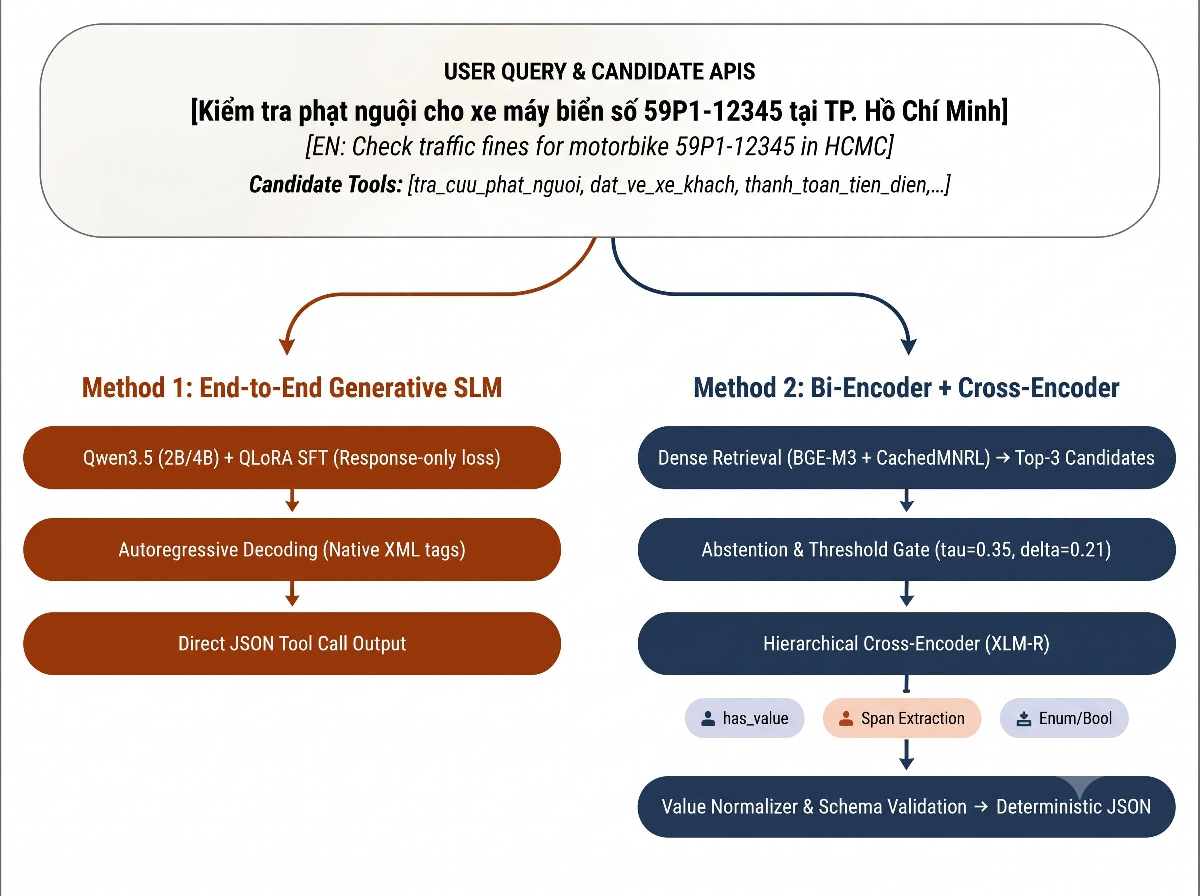
\includegraphics[width=0.88\textwidth]{figures/fig1_system_architecture}
    \caption{Sơ đồ kiến trúc đối chiếu giữa Phương pháp 1 và Phương pháp 2}
    \label{fig:hình_4_1}
\end{figure}

\textit{Hình 4.1: Sơ đồ kiến trúc đối chiếu giữa Phương pháp 1 (SLM End-to-End) và Phương pháp 2 (Bi-Encoder + Cross-Encoder).}

\section{Phương pháp 1: SLM End-to-End dựa trên Qwen3.5 (2B và 4B)}
Phương pháp 1 tiếp cận bài toán theo trường phái tạo sinh nguyên khối (End-to-End Generative Approach). Trong mô hình này, mạng nơ-ron tiếp nhận toàn bộ định nghĩa các công cụ khả dụng cùng câu truy vấn của người dùng trong cùng một cửa sổ ngữ cảnh duy nhất. Cơ chế tự chú ý (Self-Attention) cho phép mô hình liên kết trực tiếp các điều kiện ràng buộc trong mô tả API với các thực thể trong câu hỏi, từ đó tự hồi quy sinh ra cấu trúc lệnh gọi công cụ theo định dạng XML chuẩn của họ mô hình Qwen3.5:

\begin{verbatim}
<tool_call>
<function=tra_cuu_phat_nguoi>
<parameter=bien_so>30A-999.88</parameter>
<parameter=loai_phuong_tien>o_to</parameter>
</function>
</tool_call>
\end{verbatim}
Khi câu truy vấn chỉ mang tính giao tiếp thông thường hoặc không có công cụ nào trong hệ thống đáp ứng được yêu cầu, mô hình sẽ trực tiếp sản sinh câu trả lời bằng ngôn ngữ tự nhiên và từ chối tạo lập thẻ \texttt{<tool_call>}. Cơ chế này giúp hợp nhất năng lực đàm thoại tự nhiên và khả năng gọi hàm vào một mô hình thống nhất.

\textbf{Quy trình huấn luyện và thiết lập siêu tham số}:
Mô hình được tinh chỉnh trên hạ tầng GPU NVIDIA A100-40GB thông qua thư viện Unsloth và chuẩn kỹ thuật QLoRA 4-bit với các siêu tham số được mô tả chi tiết tại Bảng 4.1.


\begin{table}[htbp]
    \centering
    \caption{Thiết lập siêu tham số huấn luyện mô hình SLM Qwen3.5 (2B và 4B)}
    \label{tab:bảng_4_1}
    \begin{tabular}{lcc}
        \toprule
        \textbf{Siêu tham số (Hyperparameter)} & \textbf{Qwen3.5-2B} & \textbf{Qwen3.5-4B} \\
        \midrule
        \textbf{Kỹ thuật lượng tử hóa (Quantization)} & 4-bit NormalFloat (NF4) & 4-bit NormalFloat (NF4) \\
        \textbf{Hạng thích ứng LoRA ($r$)} & 16 & 16 \\
        \textbf{Hệ số tỷ lệ LoRA ($\alpha$)} & 16 & 16 \\
        \textbf{Target Modules} & Toàn bộ Q, K, V, O, Gate, Up, Down Proj & Toàn bộ Q, K, V, O, Gate, Up, Down Proj \\
        \textbf{Tốc độ học (Learning Rate)} & $5 \times 10^{-7}$ & $5 \times 10^{-7}$ \\
        \textbf{Bộ lập lịch tốc độ học (Scheduler)} & Cosine decay & Cosine decay \\
        \textbf{Batch Size cấu hình} & $64 \times 1$ (Per-device: 64, Accum: 1) & $32 \times 2$ (Per-device: 32, Accum: 2) \\
        \textbf{Batch Size hiệu dụng (Effective BS)} & \textbf{64} (Đồng nhất 100\%) & \textbf{64} (Đồng nhất 100\%) \\
        \textbf{Thuật toán tối ưu (Optimizer)} & AdamW 8-bit (\texttt{adamw_8bit}) & AdamW 8-bit (\texttt{adamw_8bit}) \\
        \textbf{Tỷ lệ khởi động ấm (Warmup Ratio)} & $0.05$ ($5\%$) & $0.05$ ($5\%$) \\
        \textbf{Hệ số tắt dần LoRA (Dropout)} & $0.0$ & $0.0$ \\
        \textbf{Độ dài ngữ cảnh tối đa (Max Length)} & $2{,}048$ tokens & $2{,}048$ tokens \\
        \textbf{Định dạng dữ liệu tính toán} & bfloat16 (BF16) & bfloat16 (BF16) \\
        \textbf{Kỹ thuật Gradient Checkpointing} & Kích hoạt (Unsloth Fast Gradient) & Kích hoạt (Unsloth Fast Gradient) \\
        \textbf{Tính toán hàm mất mát (Loss Masking)} & Chỉ tính trên phản hồi của Assistant & Chỉ tính trên phản hồi của Assistant \\
        \bottomrule
    \end{tabular}
\end{table}

Hệ thống siêu tham số trên được áp dụng đồng bộ và nhất quán xuyên suốt các chu trình huấn luyện (từ các cấu hình thực nghiệm đơn ngữ E1, E2 đến cấu hình song ngữ E3 và thích ứng miền chuyên biệt E4), bảo đảm tính kiểm soát biến số và khả năng đối sánh khách quan giữa các giai đoạn nghiên cứu.

\section{Phương pháp 2: Kiến trúc Phân tách Bi-Encoder + Cross-Encoder}

Phương pháp 2 chia bài toán thành hai giai đoạn: Bi-Encoder truy hồi công cụ theo ngữ nghĩa và Cross-Encoder trích xuất tham số theo lược đồ. Thiết kế mô-đun cho phép đánh giá riêng từng thành phần. Đầu ra được kiến tạo từ schema nên không ghi nhận lỗi cú pháp trong protocol hiện tại; độ trễ P50 tăng từ 55.13 ms tại $N=3$ lên 107.68 ms tại $N=1000$ trong stress test.

\section{1. Module Truy hồi Công cụ Ngữ nghĩa (Semantic Tool Retriever)}
Module đầu tiên chịu trách nhiệm thu hẹp không gian tìm kiếm từ kho hàng nghìn công cụ xuống một tập ứng viên rút gọn. Nhóm nghiên cứu sử dụng kiến trúc mạng hai tháp (Bi-Encoder) dựa trên nền tảng mô hình nhúng đa ngôn ngữ \texttt{BAAI/bge-m3}. Quá trình tối ưu hóa mô hình được triển khai thông qua quy trình huấn luyện hai vòng (two-round training): vòng thứ nhất huấn luyện mô hình cơ sở (teacher model) với hàm mất mát xếp hạng đa mẫu âm tính có bộ đệm (\texttt{CachedMNRL}); vòng thứ hai thực hiện khai thác các mẫu âm tính khó (hard negative mining) từ chính các dự đoán sai lệch của vòng 1 để tái huấn luyện mô hình cuối cùng.

Nhằm kiểm soát khả năng từ chối gọi công cụ đối với các câu hội thoại thông thường, hệ thống tích hợp cơ chế hiệu chuẩn ngưỡng kép (dual-threshold calibration) dựa trên điểm tương đồng ngữ nghĩa. Trong run Shared E4, ngưỡng tuyệt đối được hiệu chuẩn là $\tau = 0.35$ và ngưỡng biên tương đối là $\delta = 0.21$. Một công cụ mục tiêu chỉ được chấp thuận kích hoạt khi điểm tương đồng cao nhất thỏa mãn $s_{\max} \ge \tau$ và khoảng cách giữa điểm tương đồng Top-1 so với Top-2 đạt $s_{\text{top1}} - s_{\text{top2}} \ge \delta$. Các trường hợp không thỏa điều kiện được dự đoán là No-call.

\section{2. Module Trích xuất Tham số Phân cấp (Hierarchical Parameter Extractor)}
Sau khi công cụ mục tiêu được xác định, module thứ hai tiếp nhận chuỗi truy vấn của người dùng cùng với lược đồ thuộc tính (Tool Schema) của công cụ đó để trích xuất các giá trị tham số tương ứng. Module được xây dựng trên nền tảng mô hình biến đổi đa ngôn ngữ \texttt{xlm-roberta-base} với kiến trúc đầu ra phân cấp theo định hướng schema (Schema-driven routing).

Hệ thống sử dụng metadata của schema để định tuyến theo kiểu tham số. Đầu \texttt{has_value} dự đoán tham số có xuất hiện hay không; nếu có, \texttt{span_head}, \texttt{enum_head} hoặc \texttt{bool_head} xử lý theo kiểu dữ liệu tương ứng. Cơ chế giới hạn miền đầu ra cho enum và boolean, nhưng lỗi định tuyến hoặc dự đoán vẫn có thể khiến giá trị cuối cùng sai so với nhãn chuẩn.

\textbf{Quy chuẩn dữ liệu huấn luyện và hiệu chuẩn Method 2 (Shared E4)}:
Phương pháp 2 dùng cùng nguồn ngữ liệu hội thoại Shared E4 với SLM, gồm $65{,}600$ bản ghi gốc ($30{,}000$ EN, $30{,}000$ VI và $5{,}600$ CustomTools-VI Seen). Hai kiến trúc chuyển đổi bản ghi thành ví dụ huấn luyện khác nhau, nên việc dùng chung nguồn dữ liệu không bảo đảm mọi điều kiện huấn luyện và đo lường tương đương.

Trong khâu huấn luyện Bi-Encoder (\texttt{BAAI/bge-m3} tích hợp LoRA $r=16, \alpha=32$), hệ thống trích xuất chính xác $70{,}988$ cặp dương tính \texttt{(query, tool_description)} để lan truyền gradient tối ưu hóa hàm mất mát \texttt{CachedMNRL}. Toàn bộ 20 công cụ thuộc tập \texttt{unseen} bị loại trừ nghiêm ngặt khỏi dữ liệu huấn luyện dương tính, âm tính ngẫu nhiên cũng như quy trình khai thác mẫu âm khó nhằm duy trì tính độc lập hoàn toàn của miền zero-shot (\textit{Strict Zero-Shot Isolation}). Các mẫu không kích hoạt công cụ (no-call) không tham gia tính toán gradient thứ hạng mà được bảo lưu độc lập phục vụ cho việc hiệu chuẩn bộ tham số ngưỡng quyết định ($\tau = 0.35, \delta = 0.21$) trên tập kiểm định.

Đối với khâu huấn luyện Cross-Encoder (\texttt{xlm-roberta-base} với kiến trúc Hierarchical Heads), ngữ liệu được phân rã thành $135{,}617$ cặp \texttt{(query, param_schema)} gióng hàng trực tiếp, phục vụ huấn luyện liên hợp đầu nhị phân \texttt{has_value} và ba nhánh phân cấp chuyên biệt. Quy trình kiểm thử đối chuẩn sau đó được triển khai đồng bộ trên toàn bộ $7{,}712$ mẫu kiểm thử Core tiếng Việt (gồm $7{,}221$ mẫu có lệnh gọi và $491$ mẫu âm tính), $7{,}712$ mẫu Core tiếng Anh và hai tập kiểm thử \texttt{CustomTools-VI} Seen/Unseen với mỗi tập $800$ mẫu cân bằng 50\% âm tính.

Chi tiết toàn bộ cấu hình siêu tham số và tài nguyên tính toán của Phương pháp 2 được tổng hợp tại Bảng 4.2.


\begin{table}[htbp]
    \centering
    \caption{Thiết lập siêu tham số huấn luyện Phương pháp 2 (BGE-M3 và XLM-R)}
    \label{tab:bảng_4_2}
    \begin{tabular}{lll}
        \toprule
        \textbf{Thành phần kỹ thuật} & \textbf{Bộ truy hồi Bi-Encoder (BGE-M3)} & \textbf{Bộ trích xuất Cross-Encoder (XLM-R)} \\
        \midrule
        \textbf{Kiến trúc mô hình gốc} & \texttt{BAAI/bge-m3} (Dense Bi-Encoder) & \texttt{xlm-roberta-base} (Hierarchical Cross-Encoder) \\
        \textbf{Kỹ thuật thích ứng (PEFT)} & LoRA ($r=16, \alpha=32$, dropout $0.05$) & Huấn luyện liên hợp toàn diện (End-to-End Head Tuning) \\
        \textbf{Target Modules (LoRA)} & \texttt{query}, \texttt{key}, \texttt{value}, \texttt{dense} & — \\
        \textbf{Chiều dài chuỗi tối đa} & 192 tokens & 256 tokens (Question: 96, Context: 160) \\
        \textbf{Kích thước Batch (Batch size)} & 256 (Mini-batch: 32) & 32 (Gradient Accumulation Steps: 2 $\to$ 64) \\
        \textbf{Tốc độ học (Learning Rate)} & $2 \times 10^{-5}$ & Core: $3 \times 10^{-5}$, Custom: $1 \times 10^{-5}$, Heads: $1 \times 10^{-4}$ \\
        \textbf{Chiến lược huấn luyện} & 2 Rounds (Round 1 Teacher $\to$ Hard Negative Mining) & Curriculum Learning (2 Epochs Core $\to$ 2 Epochs Custom) \\
        \textbf{Hàm mất mát (Loss function)} & \texttt{CachedMultipleNegativesRankingLoss} & Binary Cross-Entropy (\texttt{has_value}, \texttt{bool}) + Cross-Entropy (\texttt{span}, \texttt{enum}) \\
        \textbf{Quy chuẩn quyết định (Policy)} & Gap selection: $\tau = 0.35, \delta = 0.21, k_{\max} = 3$ & Schema-driven routing + Regex Value Normalizer \\
        \textbf{Thời gian huấn luyện (Tesla T4)} & 6.15 giờ (Round 2 trên $70{,}988$ cặp dương tính) & 0.72 giờ ($4{,}240$ bước tối ưu hóa trên $135{,}617$ cặp) \\
        \textbf{Đỉnh chiếm dụng VRAM huấn luyện} & $10{,}888$ MB & $7{,}693$ MB \\
        \bottomrule
    \end{tabular}
\end{table}

\section{Cơ chế chuẩn hóa giá trị thực thể tiếng Việt (Vietnamese Value Normalizer)}

Đầu \texttt{span_head} của Cross-Encoder trích chuỗi xuất hiện trong truy vấn, còn API yêu cầu giá trị đúng kiểu và định dạng theo JSON Schema. Chẳng hạn, chuỗi \texttt{"hai triệu rưỡi"} không thể dùng trực tiếp cho tham số kiểu số. Vì vậy, Method 2 cần bước chuyển đổi giá trị trước khi tạo lời gọi.

Module Chuẩn hóa Giá trị tiếng Việt (Vietnamese Value Normalizer) sử dụng các quy tắc xác định qua bốn giai đoạn:

Giai đoạn 1 tách các biểu thức định lượng và ánh xạ từ lóng tiền tệ: “củ”, “chai” tương ứng $10^6$ đồng; “lít”, “xị”, “loét” tương ứng $10^5$ đồng; “cành”, “k” tương ứng $10^3$ đồng. Từ “rưỡi” biểu thị nửa đơn vị đứng trước, nên “hai củ rưỡi” được chuẩn hóa thành $2{,}500{,}000$ đồng.

Giai đoạn 2 phân tích số viết bằng chữ tiếng Việt theo thứ bậc tỷ, triệu, nghìn, trăm và hàng chục. Bộ phân tích cũng xử lý các biến thể như “lăm”, “nhăm”, “mươi” và “chục” để trả về giá trị số.

Giai đoạn 3 chuẩn hóa ngày tháng và mã định danh có cấu trúc. Các biểu thức thời gian được quy về ngày tuyệt đối theo thời điểm neo của hệ thống và định dạng ISO-8601 (\texttt{YYYY-MM-DD}). Với biển số và mã giao dịch, các quy tắc biểu thức chính quy xử lý khoảng trắng, dấu gạch ngang và chữ hoa; ví dụ, \texttt{"59 x1 999.88"} thành \texttt{"59X1-999.88"}.

Giai đoạn 4 ép giá trị theo kiểu khai báo tại \texttt{tools[].parameters.properties[key].type}, gồm \texttt{int}, \texttt{float}, \texttt{bool} hoặc chuỗi đã làm sạch. Đầu ra vẫn cần được xác thực theo JSON Schema trước khi thực thi; tỷ lệ lỗi cú pháp 0\% không có nghĩa là mọi tham số đều đúng nhãn chuẩn.

Hình 4.2 tóm tắt bốn giai đoạn xử lý.

\begin{verbatim}
graph LR
    classDef io fill:#e1f5fe,stroke:#0288d1,stroke-width:2px,color:#01579b;
    classDef step fill:#f3e5f5,stroke:#7b1fa2,stroke-width:2px,color:#4a148c;

    Raw["Chuỗi văn bản thô trích xuất từ span_head"]:::io
    S1["Bước 1: Phân đoạn từ vựng & Ánh xạ từ lóng<br/>('hai củ rưỡi' -> 2,500,000, 'năm xị' -> 500,000)"]:::step
    S2["Bước 2: Phân tích cú pháp số chữ tiếng Việt<br/>(Giải mã đệ quy hàng đơn vị, chục, trăm, triệu)"]:::step
    S3["Bước 3: Chuẩn hóa Regex có cấu trúc<br/>(Định dạng biển số xe, ngày tháng ISO-8601)"]:::step
    S4["Bước 4: Áp đặt kiểu dữ liệu theo Schema<br/>(Ép kiểu nguyên thủy integer, float, bool, string)"]:::step
    Clean["Giá trị tham số chuẩn hóa (JSON Compliant)"]:::io

    Raw --> S1
    S1 --> S2
    S2 --> S3
    S3 --> S4
    S4 --> Clean
\end{verbatim}

\textit{Hình 4.2: Quy trình bốn giai đoạn của module Chuẩn hóa Giá trị tiếng Việt (Vietnamese Value Normalizer).}

